\chapter{Implementation}\label{ch:impl}

\section{Built drones}

In total, four full-assembled drones were built for this project using the hardware described in Chapter \ref{ch:hw}: two model-A units and two model-B, both models shown in Figures \ref{fig:imp_models_noCover} and \ref{fig:imp_modelsFULL}. The four drones are shown in Figure \ref{fig:imp_4drones}, and they are separated in two groups: the drones that belong to AAU (one model-A and one model-B) and the ones that belong to DTU (also one model-A and one model-B). Each group of drones has a single transmitter, that can be paired with any receiver of the drones.

Additionally, there are two not-assembled spare sets and each set has a FPGA, a PCB, a cover, a FPGA-frame attachment, a frame and the sensors that are attached on top of the PCB.


\begin{figure} [H]
    \centering
    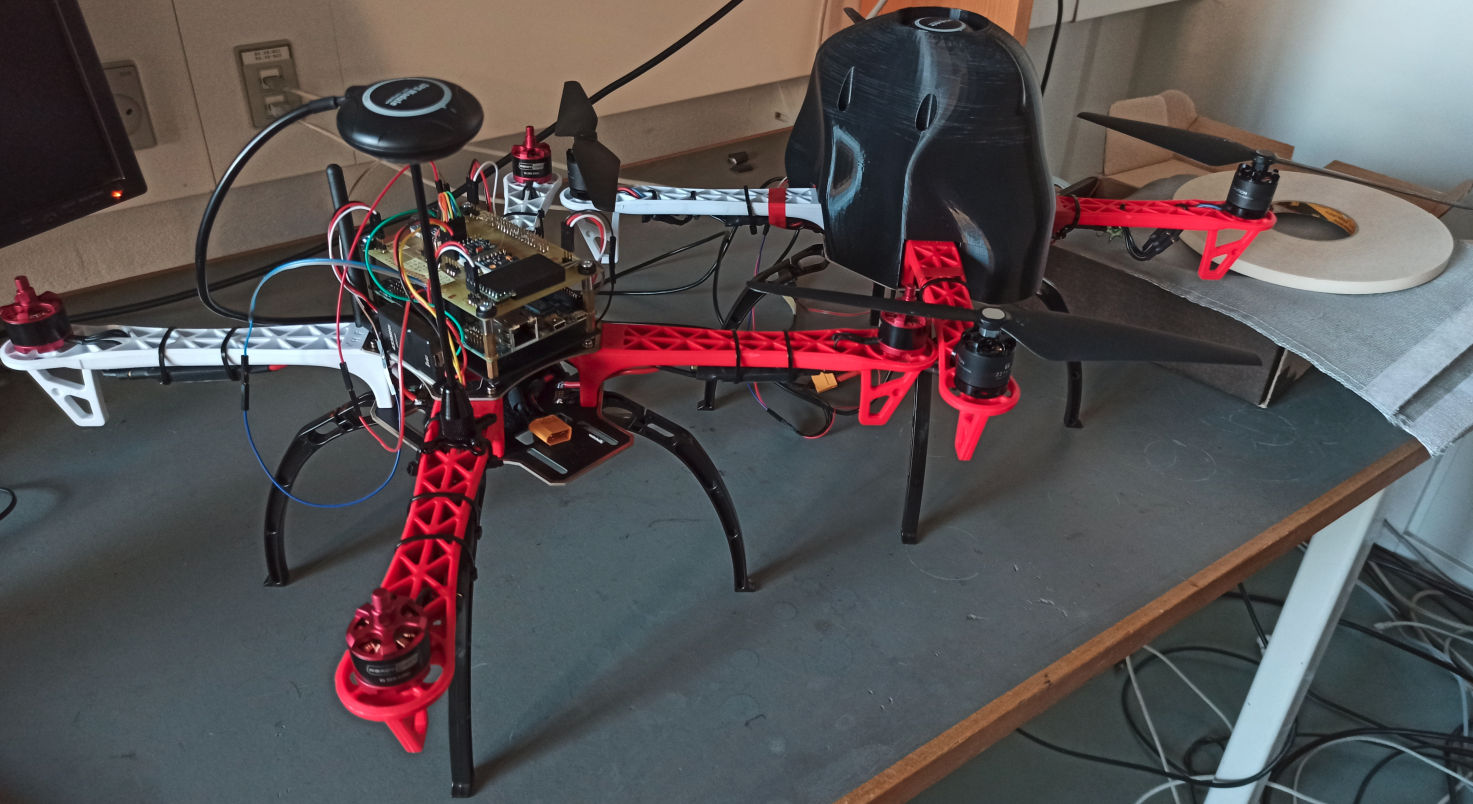
\includegraphics[width=\textwidth]{Figures/implementation/modelA_and_B.png}
    \caption{Model-A without cover (left) and Model-B (right). Both units have inside a FPGA with a PCB attached as shown.}
    \label{fig:imp_models_noCover}
\end{figure}

\begin{figure} [H]
    \centering
    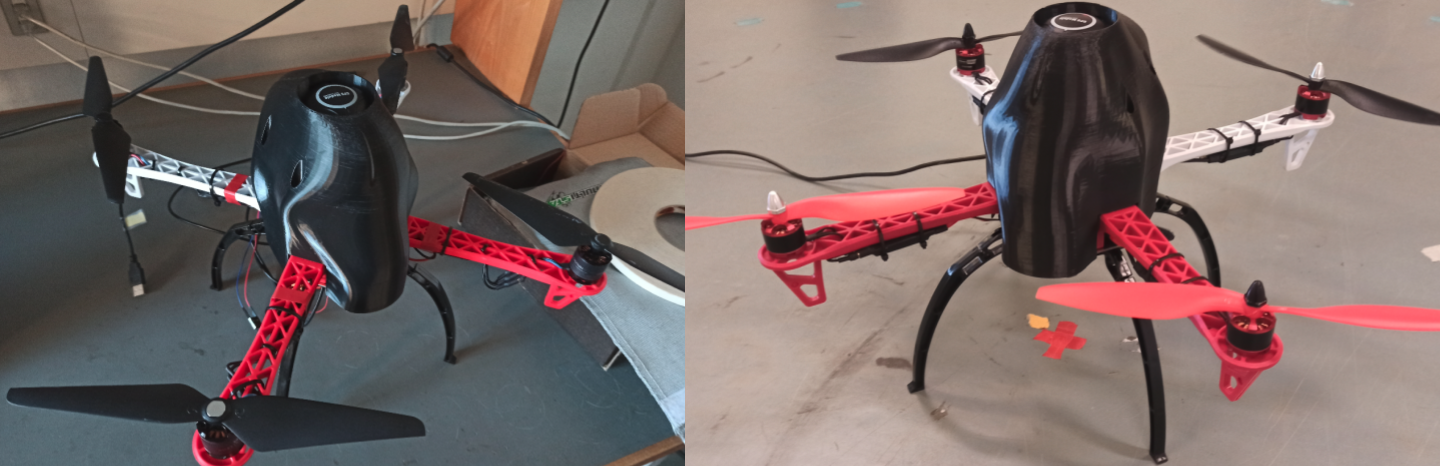
\includegraphics[width=\textwidth]{Figures/implementation/modelA_and_B_assembled.png}
    \caption{Fully assembled Model-B (left) and A (right) units.}
    \label{fig:imp_modelsFULL}
\end{figure}


\begin{figure} [H]
    \centering
    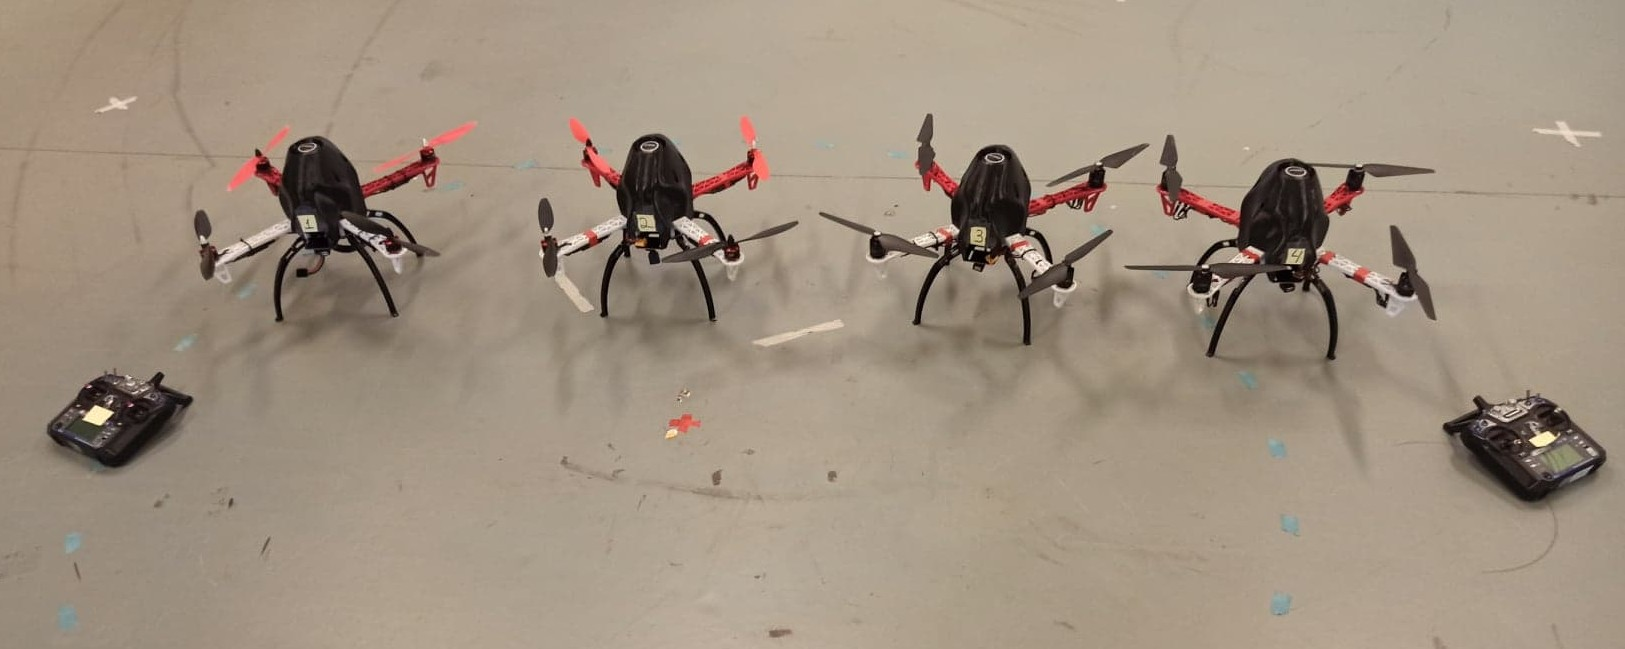
\includegraphics[width=\textwidth]{Figures/implementation/four_drones_tel.jpg}
    \caption{From left to right: AAU transmitter, drone 1 (Model-A, group AAU), drone 2 (Model-A, group DTU), drone 3 (Model-B, group AAU), drone 4 (Model-B, group DTU), DTU transmitter. Next to each drone, there is its paired telemetry module for a remote station.}
    \label{fig:imp_4drones}
\end{figure}


\section{Patmos configuration}

The Patmos architecture for this project is called de10-nano-drone and its configuration is quite different from the standard de10-nano or the default configurations. Here are some its hardware specifications:

\begin{itemize}
    \item ADC Module: This resource is available inside the FPGA and hard-wired to it. This module has its own set of pins for the analog inputs and its separate power supply.
    \item I2C Master for multiple sensors: the SDA and SCL pins work as a bus to connect three different sensors (IMU, barometer, compass).
    \item Second and third UART ports: the second UART has the same baud rate as the GPS and the third UART has the same baud rate as the telemetry module and a bigger FIFO depth for longer messages exchange.
    \item Modification on Actuators: it works as an input and it has 6 pins, so it is used for the 6-channels receiver.
    \item External memory of 1GB: it uses the micro SD card from the FPGA. This is required for the multi-core feature.
    \item Multi-core assignment: there are 4 cores in use and the devices must be assigned to a core (by default they are assigned to core nr.0). The devices have been assigned as it follows:
    \begin{itemize}
        \item Core 0: ADC module and LEDs.
        \item Core 1: I2C master.
        \item Core 2: Actuators (receiver), and this also includes Propulsion (motors).
        \item Core 3: UART 2 and 3.
    \end{itemize}
\end{itemize}


\section{Software architecture}

The flight controller algorithm and functionalities described on the previous Chapter \ref{ch:sw} have been implemented as an application written in C. This implementation is divided in different groups of scripts and header files. As shown in Figure \ref{fig:imp_arch}, there are six groups:

\begin{itemize}
    \item Basic functionalities: it contains all the low-level and hardware-related dependencies.
    \item Components: using the basic functionalities, it implements the full functionalities of the devices and they are meant for the specific components from the Tables \ref{tab:comp_common} and \ref{tab:comp_AB}.
    \item Flying functionalities and flight controller: they contain the different modes and the flight algorithm described on Section \ref{sec:general_working}.
    \item Test programs: it implements different test scripts for checking the functionality of every device. Every program is described in Chapter \ref{ch:test}.
    \item Simulation: it contains the simulation scripts, dependencies and simulation scenes, which are described in Section \ref{sec:simulation}
\end{itemize}

\begin{figure} [H]
    \centering
    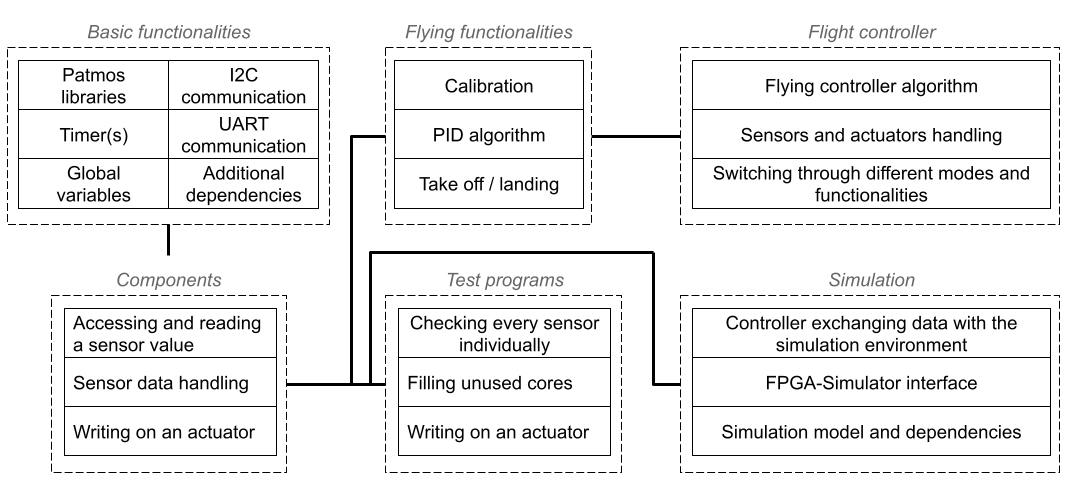
\includegraphics[width=\textwidth]{Figures/implementation/fc_architecture.png}
    \caption{Software architecture for the flight controller and additional functionalities.}
    \label{fig:imp_arch}
\end{figure}

%\vfill % <- use this to avoid big blank spaces
%\clearpage
%\newpage
% Start on a new page
\section{Drone simulation}\label{sec:simulation}

Another concept for the project was to develop a simulation model of the drone that can be used for testing the flight controller while running on the FPGA. The main idea for this approach is shown in Figure \ref{fig:sim_concept} and it can be described as follows:

\begin{itemize}
    \item The goal is to simulate and find bugs on the flight controller, so the simulation aims to test the drone on the fly and how it reacts to changes on the commands from the pilot through the transmitter. Thus the actual FPGA, receiver and transmitter are needed, as shown in Figure \ref{fig:sim_setup}.
    
    \item The Patmos architecture and a modified version of the flight controller are downloaded on the board.
    
    \item The modified version of the flight controller uses the telemetry port to exchange messages with the simulator. It gets all the sensors values required (IMU, barometer, GPS,...) from the messages instead of using their normal ports (I2C, UART1).
    
    \item On the PC Station, it is needed a program that works as an interface between the FPGA and the simulator, which was implemented as a Python script. This interface access the port where the UART2 is sending/receiving messages and the simulation drone. In the run, it gets the sensors values, converts them to the same format as the real ones and sends them to the FPGA. On the other hand, it gets the motor commands from the FPGA and converts them into the units that the simulation drone works with (in this case $rad/s$) and sends it to the simulation.
    
\end{itemize}

\begin{figure} [H]
    \centering
    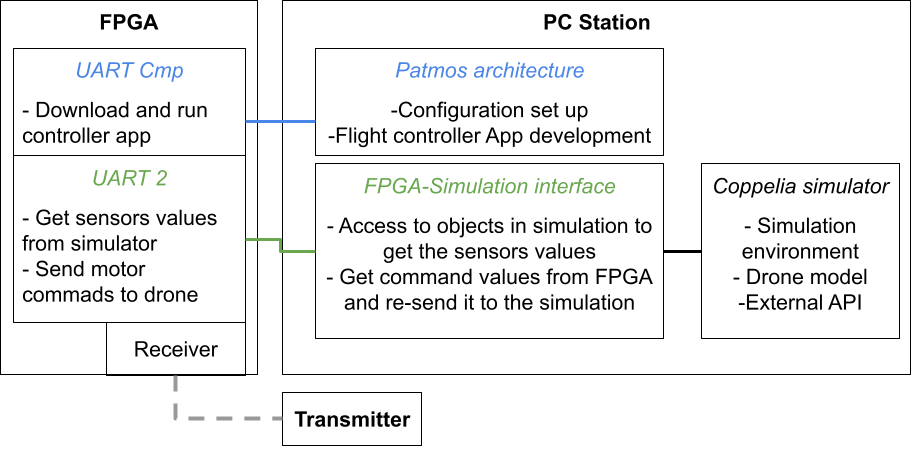
\includegraphics[width=\textwidth]{Figures/simulation/simulation_concept.png}
    \caption{Simulation diagram}
    \label{fig:sim_concept}
\end{figure}

\begin{figure} [H]
    \centering
    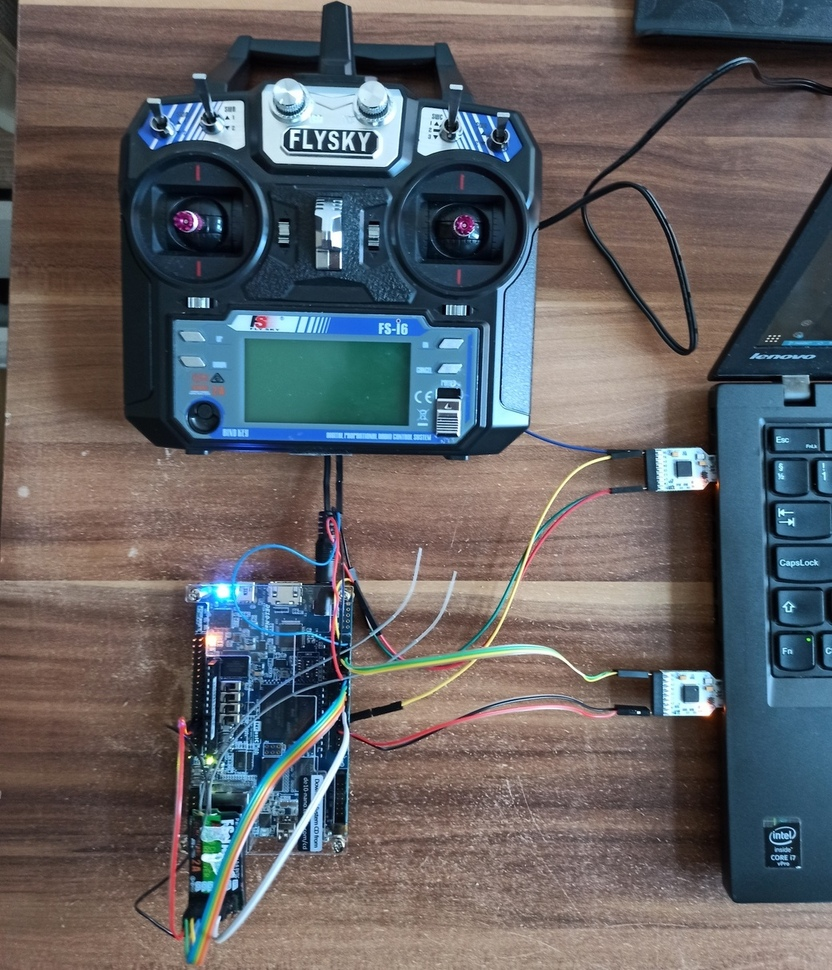
\includegraphics[scale=0.3]{Figures/simulation/simulation_setup.jpg}
    \caption{Simulation set up: transmitter (top left), FPGA with a receiver, two UART-USB adapters (connected to UART Cmp and UART2), and a laptop (right).}
    \label{fig:sim_setup}
\end{figure}

The drone model presented in \ref{sec:hw_mec} can be exported from SolidWorks into Universal Robot Description Format (URDF) \cite{bib:urdfPlugin}. Thus, the simulator chosen is CoppeliaSim, which is compatible with this format.

Both Model-A and Model-B were successfully imported into CoppeliaSim and added to the simulator library as robot models, as shown in Figure \ref{fig:sim_models}. On top of that, the models from Solidworks do not include the sensors and these had to be added manually on the simulated models. A successful test showed that the communication between the different elements was possible and the program interface could exchange messages with the FPGA and get values from the sensors on the simulation.s

However, the CoppeliaSim simulator does not have fluid mechanics on the physics engine, so the simulation environment is on a vacuum space. In order to make a mobile robot move within a 3D space, it is necessary to implement on the simulation scrips the differential equations and forces that must be applied on the body. 

There are another mobile robot models within the models library that have managed to successfully implement this (another quad-copter drone and a swimming snake robot), but this was not achieved for this project. Both drone models were set as dynamic and responsive objects and they can spin their motors, but they cannot take off properly. Finally, this part of the project remains unfinished due to the fact that the real lab and components were accessible.

\begin{figure} [H]
    \centering
    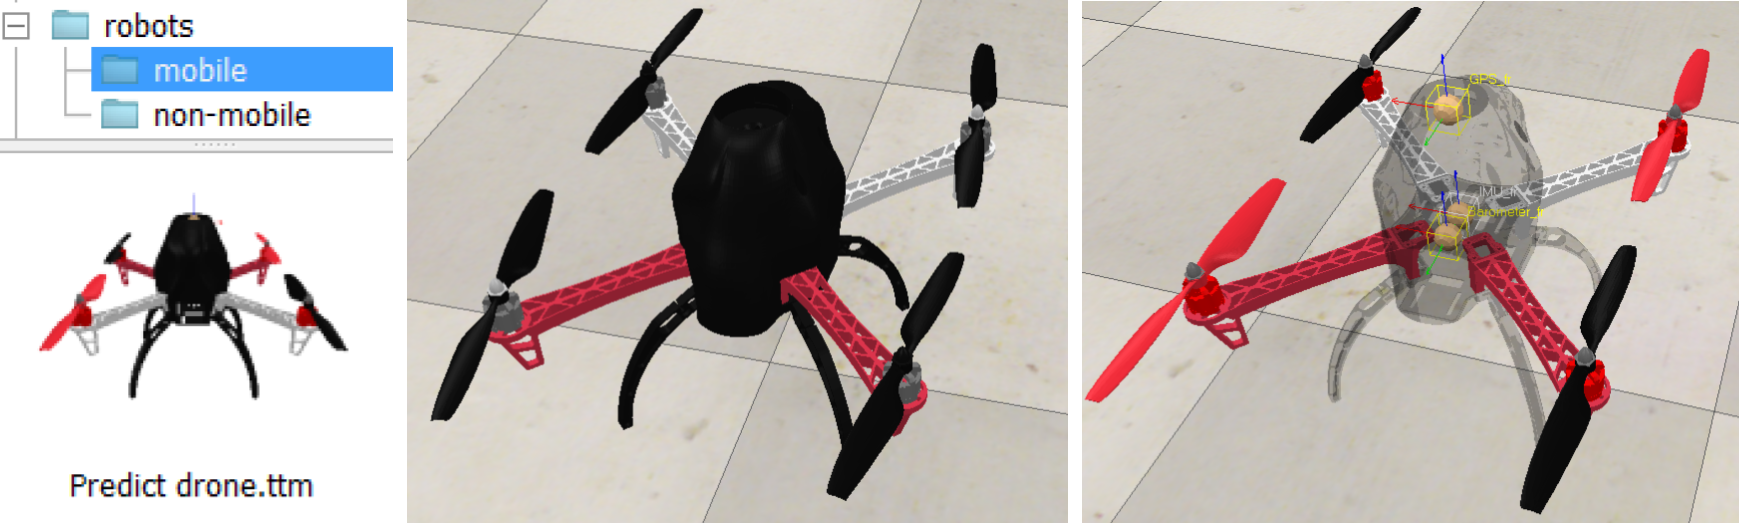
\includegraphics[width=\textwidth]{Figures/simulation/coppelia_model.png}
    \caption{From left to right: drone model imported and saved in Coppelia library, a drone frame in simulation (example with a Model-B), showing the inside of the cover where the sensors had to be added to the simulation model (example with a Model-A).}
    \label{fig:sim_models}
\end{figure}
